\documentclass[12pt]{article}

%%%%% Document Information (FILL THIS IN!) %%%%%
\newcommand{\authornames}{(Names)}

\newcommand{\coursenumber}{CSC 341}
\newcommand{\assignmentname}{Daily Exercises \#18}
\newcommand{\assignmentversion}{1}

%%%%% Fonts and Encodings %%%%%%%%%%%%%%%%%%%%%%%%%%%%%%%%%%%%%%%%%%%%%%%%%%%%%%
\usepackage[T1]{fontenc}
\usepackage{libertine}

%%%%% General %%%%%%%%%%%%%%%%%%%%%%%%%%%%%%%%%%%%%%%%%%%%%%%%%%%%%%%%%%%%%%%%%%
\usepackage{amsmath}
\usepackage{amssymb}
\usepackage{enumitem}
\usepackage{fancyvrb}
\usepackage[amsmath, amsthm, thmmarks]{ntheorem}
\usepackage{microtype}
\usepackage{url}
\usepackage[svgnames]{xcolor}
\usepackage{xspace}

\usepackage{tikz}

%%%%% Page Formatting %%%%%%%%%%%%%%%%%%%%%%%%%%%%%%%%%%%%%%%%%%%%%%%%%%%%%%%%%%
\usepackage[
  top=1in,
  bottom=1in,
  left=1in,
  right=1in,
  includefoot,
  paperwidth=8.5in,
  paperheight=11in
]{geometry}

\usepackage{fancyhdr}
\setlength{\headheight}{15.2pt}
\pagestyle{fancy}

\fancyhead{}
\fancyfoot{}
\lhead{\coursenumber{}---\assignmentname{} (ver. \assignmentversion), \authornames{}}
\cfoot{\thepage}

%%%%% Code %%%%%%%%%%%%%%%%%%%%%%%%%%%%%%%%%%%%%%%%%%%%%%%%%%%%%%%%%%%%%%%%%%%%%

\usepackage{listings}
\usepackage{xcolor}

% Adapted from: https://en.wikibooks.org/wiki/LaTeX/Source_Code_Listings
\definecolor{mygreen}{rgb}{0,0.6,0}
\definecolor{mygray}{rgb}{0.5,0.5,0.5}
\definecolor{mymauve}{rgb}{0.58,0,0.82}

\lstset{ 
  backgroundcolor=\color{white},      % choose the background color; you must add \usepackage{color} or \usepackage{xcolor}; should come as last argument
  basicstyle=\ttfamily\footnotesize,  % the size of the fonts that are used for the code
  breakatwhitespace=false,            % sets if automatic breaks should only happen at whitespace
  breaklines=true,                    % sets automatic line breaking
  captionpos=b,                       % sets the caption-position to bottom
  commentstyle=\color{mygreen},       % comment style
  keepspaces=true,                    % keeps spaces in text, useful for keeping indentation of code (possibly needs columns=flexible)
  keywordstyle=\color{blue},          % keyword style
  language=Java,                      % the language of the code
  stringstyle=\color{mymauve},        % string literal style
}

%%%%% Basic Macros and Definitions %%%%%%%%%%%%%%%%%%%%%%%%%%%%%%%%%%%%%%%%%%%%%
\newtheorem{claim}{Claim}
\newtheorem{invariant}{Invariant}
\newtheorem{defn}{Definition}
\newtheorem{thm}{Theorem}
\newtheorem{lemma}{Lemma}

\newcommand{\ie}{\emph{i.e.}\xspace}
\newcommand{\eg}{\emph{e.g.}\xspace}
\newcommand{\hint}[1]{(\emph{Hint}: #1)}

\newcounter{ProblemCounter}
\newenvironment{problem}[1][]
  {\refstepcounter{ProblemCounter}\noindent\textbf{Problem \theProblemCounter{} (#1)}\quad}
  {\newpage}

\newcommand{\answerbelow}{\noindent\makebox[\linewidth]{\rule{\textwidth}{0.4pt}}}


%%%%% Problem-specific Macros %%%%%%%%%%%%%%%%%%%%%%%%%%%%%%%%%%%%%%%%%%%%%%%%%%

\newcommand{\np}{\ensuremath{\mathsf{NP}}\xspace}
\newcommand{\pspace}{\ensuremath{\mathsf{PSPACE}}\xspace}
\newcommand{\prob}[1]{\ensuremath{\textsf{#1}}\xspace}
\newcommand{\desc}[1]{\ensuremath{\langle #1 \rangle}}
\newcommand{\Nat}{\ensuremath{\mathbb{N}}\xspace}
\newcommand{\comp}[1]{\ensuremath{\overline{#1}}\xspace}

%%%%%%%%%%%%%%%%%%%%%%%%%%%%%%%%%%%%%%%%%%%%%%%%%%%%%%%%%%%%%%%%%%%%%%%%%%%%%%%%

\begin{document}

\begin{problem}[Puzzle Game]
  Recall the \emph{puzzle} problem, \prob{PUZZLE}, from a previous daily
  assignment.
  \begin{quote}
    You are given a box and a collection of cards as indicated in the following
    figure.  Because of the pegs in the box and the notches in the cards, each
    card will fit in the box in either of two ways.  Each card contains two
    columns of holes, some of which may not be punched out. The puzzle is solved
    by placing all the cards in the box so as to completely cover the bottom of
    the box (\ie, every hole position is blocked by at least one card that has no
    hole there).

    \begin{center}
      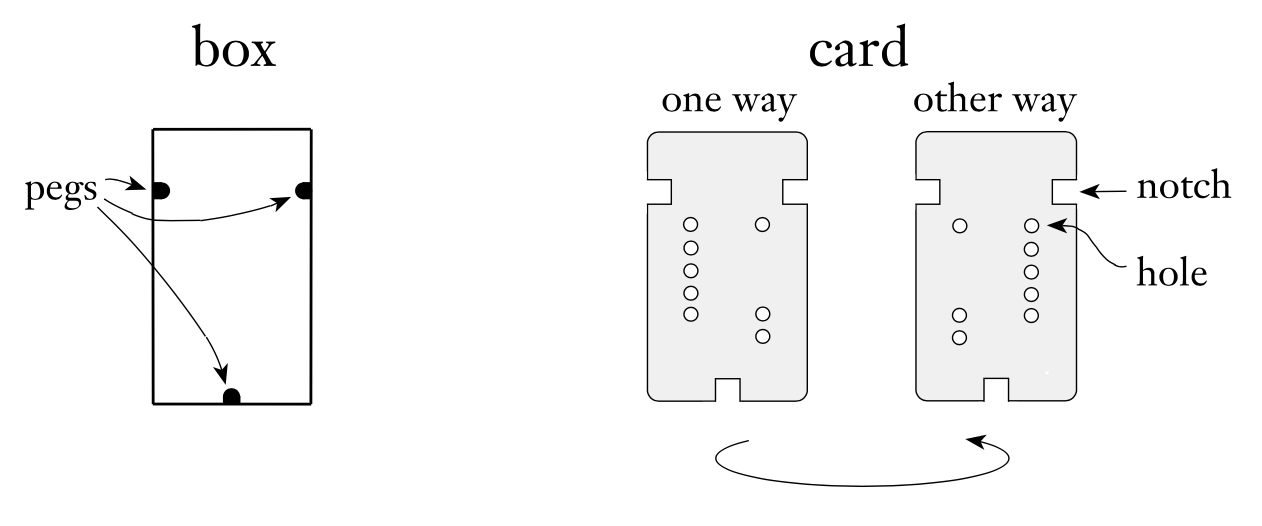
\includegraphics[width=0.75\textwidth]{cards}
    \end{center}
  \end{quote}

  Consider a related problem, the two-player \emph{puzzle game},
  \prob{PUZZLE-GAME}.  The game consists of an \emph{ordered} stack of cards as
  described in \prob{PUZZLE}.  Players take turns placing the cards in order
  into the box, choosing whether or not the card is flipped.  After placing all
  the cards, player one wins if all the hole positions are covered in the
  stack; player two wins if this is not the case.  Define:
  \[
    \prob{PUZZLE-GAME} = \{ \desc{C} \mid \text{ \( C \) is an ordered stack of puzzle cards and player 1 has a winning strategy } \}.
  \]
  In this problem, we'll show that \prob{PUZZLE{-}GAME} is \pspace-complete.
  \begin{enumerate}[itemsep=0pt]
    \item Show that \( \prob{PUZZLE-GAME} \in \pspace \).
    \item From the reading, you know that
      \[
        \prob{FORMULA-GAME} = \{ \desc{\phi} \mid \text{ \( \phi \) is a TQBF and player 1 has a winning strategy } \}.
      \]
      is \pspace-complete.  Furthermore, the restriction of the boolean
      formulas to 3-cnf form is also \pspace-complete.  Use this fact to
      construct a polynomial time mapping function from the 3-cnf version of
      \prob{FORMULA-GAME} to \prob{PUZZLE{-}GAME}, demonstrating that
      \prob{PUZZLE-GAME} is \pspace-hard.  In a few sentences, argue why your
      construction is correct.  \hint{Adopt the solution for \prob{PUZZLE}
      directly.}
    \item Show your construction is correct by giving an example of the output
      of your mapping function on the following TQBF in 3-cnf form:
      \[
        \exists x_1 \forall x_2 \exists x_3 \ldotp [ (x_1 \vee x_2 \vee x_1) \wedge (x_2 \vee x_3 \vee x_3) \wedge (\overline{x_2} \vee \overline{x_3} \vee \overline{x_3}) ]
      \]
      Use the \texttt{verbatim} environment to draw your resulting cards with
      ASCII art.
  \end{enumerate}

\answerbelow{}

% FILL IN YOUR ANSWER HERE

\end{problem}

%%%%%%%%%%%%%%%%%%%%%%%%%%%%%%%%%%%%%%%%%%%%%%%%%%%%%%%%%%%%%%%%%%%%%%%%%%%%%%%%

\end{document}
